% rubber: set program xelatex
\documentclass[18pt,mathserif]{beamer}

%{{{ Settings
\usetheme[english, titlepage0]{KIT}

%{{{ Packages
\usepackage{tikz}
%\usepackage{xltxtra}
\usepackage{csquotes}
\usepackage{caption}
\usepackage{hyperref}
\usepackage[framemethod=tikz]{mdframed}
%}}}
%{{{ Fonts and colors
%\setsansfont[Mapping=tex-text,
%             BoldFont={* Semibold}]{Source Sans Pro}
%\setmonofont[UprightFeatures={LetterSpace=-0.5}]{Inconsolata}

% TomorrowTheme: https://github.com/chriskempson/tomorrow-theme/blob/master/vim/colors/Tomorrow.vim
\definecolor{syntax-comment}{HTML}{8e908c}
\definecolor{syntax-keyword}{HTML}{8959a8}
\definecolor{syntax-number}{HTML}{eab700}
\definecolor{syntax-green}{HTML}{718c00}
\definecolor{syntax-red}{HTML}{c82829}

\setbeamercolor{section in toc}{fg=black!80}
%}}}
%{{{ TikZ styles
\usetikzlibrary{arrows, backgrounds, calc, trees, shapes, snakes}

\tikzset{
  commit/.style={
    circle, draw, color=black!75, fill=syntax-keyword!75,
    line width=1pt, minimum height=12pt
  },
  connection/.style={
    draw, ->, >=stealth, color=black!75, line width=.75pt
  }
}

\pgfdeclareimage[width=.36cm]{butthurt}{images/butthurt}

\newcommand\score[2]{
  \pgfmathsetmacro\pgfxa{#1+1}
  \begin{tikzpicture}[baseline=-3pt]
    \foreach \i in {1,...,#2} {
      \pgfmathparse{(\i<=#1?"1.0":"0.3")}
      \edef\starcolor{\pgfmathresult}
      \node[name=butthurt\i, opacity=\starcolor, inner sep=0pt] at (\i*3ex,0) {\pgfuseimage{butthurt}};
    }
  \end{tikzpicture}
}

\makeatletter
\tikzset{
  circle split part fill/.style  args={#1,#2}{%
    alias=tmp@name, % Jake's idea !!
    postaction={%
      insert path={
        \pgfextra{%
          \pgfpointdiff{\pgfpointanchor{\pgf@node@name}{center}}%
                       {\pgfpointanchor{\pgf@node@name}{east}}%
          \pgfmathsetmacro\insiderad{\pgf@x}
          \fill[#1] (\pgf@node@name.base) ([xshift=-\pgflinewidth]\pgf@node@name.east) arc
                            (0:180:\insiderad-\pgflinewidth)--cycle;
          \fill[#2] (\pgf@node@name.base) ([xshift=\pgflinewidth]\pgf@node@name.west)  arc
                            (180:360:\insiderad-\pgflinewidth)--cycle;
        }
      }
    }
  }
}
\makeatother
%}}}
%{{{ Environments
\makeatletter
\newenvironment{shell}[1][\linewidth]
  {\begin{mdframed}[
  skipabove=\topsep,
  skipbelow=\topsep,
  font=\ttfamily,
  linecolor=black!9,
  backgroundcolor=black!9,
  innertopmargin=6pt,
  innerbottommargin=6pt,
  innerleftmargin=6pt,
  innerrightmargin=6pt,
  userdefinedwidth=#1]}
  {\end{mdframed}}
\makeatother
%}}}
%{{{ Meta
\title{Distributed version control and why \emph{you} want to use it}
\author{M. Vogelgesang}
\subtitle{Matthias Vogelgesang}
\institute{Institute for Data Processing and Electronics}
\date{Oct.~17\textsuperscript{th} 2013}

\graphicspath{{../../common/}}

\TitleImage[width=6.5cm]{images/git-icon}
%}}}

%}}}

\begin{document}
\maketitle

\section{Version Control}

\begin{frame}{Plead guilty!}
  It's easy to copy digital content, so why not re-create it over and over
  again?

  \begin{columns}[onlytextwidth]
    \visible<2->{
      \column{0.5\textwidth}
        \begin{figure}
          \centering
          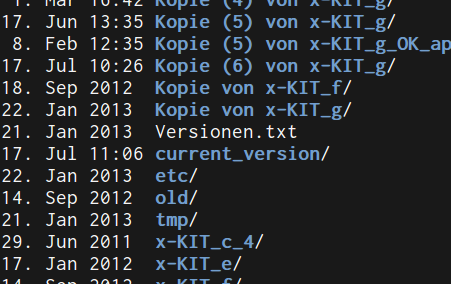
\includegraphics[width=4.5cm]{images/mrcs.png}
          \caption*{\enquote{One of these folders \emph{must} contain the latest
          version \ldots}}
        \end{figure}
    }

    \visible<3->{
      \column{0.5\textwidth}
        \begin{figure}
          \centering
          
\includegraphics[width=4.5cm]{images/reports.png}
          \caption*{\enquote{Here is the latest version of the
          proposal/paper/report.} --- \enquote{Thanks.}}
        \end{figure}
    }
  \end{columns}
\end{frame}
\begin{frame}{Obvious disadvantages}
  \begin{itemize}
    \item No meta data about \emph{what} was changed \emph{when} by
      \emph{whom}
    \item You lose track of what's going on
    \item You cannot roll-back to a working state
    \item Poor solution for collaboration
  \end{itemize}
\end{frame}
\begin{frame}{Version control}
  \begin{block}{Benefits}
    \begin{itemize}
      \item \emph{Track} files
      \item Record (\emph{commit}) changes
      \item Share changes with others
      \item Roll-back to an earlier state
    \end{itemize}
  \end{block}
\end{frame}

\section{Distributed Version Control}

\begin{frame}{Centralized version control systems}
  \begin{block}{Implementations}
    \begin{itemize}
      \item File-based: RCS
      \item Client-Server architecture: CVS, SVN, \ldots
    \end{itemize}
  \end{block}

  \pause

  \begin{block}{Problems}
    \begin{itemize}
      \item Centralized systems require a server
      \item Interaction with a repository can be painfully slow
      \item Setup and maintenance issues
      \item Collaborating requires a lot of effort
    \end{itemize}
  \end{block}
\end{frame}
\begin{frame}{Distributed version control}
  \begin{block}{Cloned repositories}
    \begin{itemize}
      \item Local setup
      \item Blazingly fast operations
      \item \enquote{Airplane coding}
    \end{itemize}
  \end{block}
  \begin{block}{Sharing is an inherent feature}
    \begin{itemize}
      \item DVCS are built around the idea of sharing
      \item Cryptographic hashing of content assures integrity
      \item Easy branching and merging of changes between peers
    \end{itemize}
  \end{block}
\end{frame}
\begin{frame}{Distributed version control \emph{systems}}
  Mercurial, Bazaar, SVK, Monotone, BitKeeper, \textbf{Git}, Darcs, Fossil, GNU
  arch, Arx, Plastic SCM
\end{frame}
\begin{frame}{Why Git?}
  \begin{columns}[T,onlytextwidth]
    \column{0.5\textwidth}
      \begin{block}{Pros}
        \begin{itemize}
          \item De-facto standard for open source software
          \item Probably the fastest DVCS out there
          \item GitHub has more sex appeal than sf.net
        \end{itemize}
      \end{block}

      \begin{block}{Cons}
        \begin{itemize}
          \item Command line interface can be a bit inconsistent
          \item Git is a toolbox with much freedom and little limits
        \end{itemize}
      \end{block}
    \column{0.5\textwidth}
      \centering
      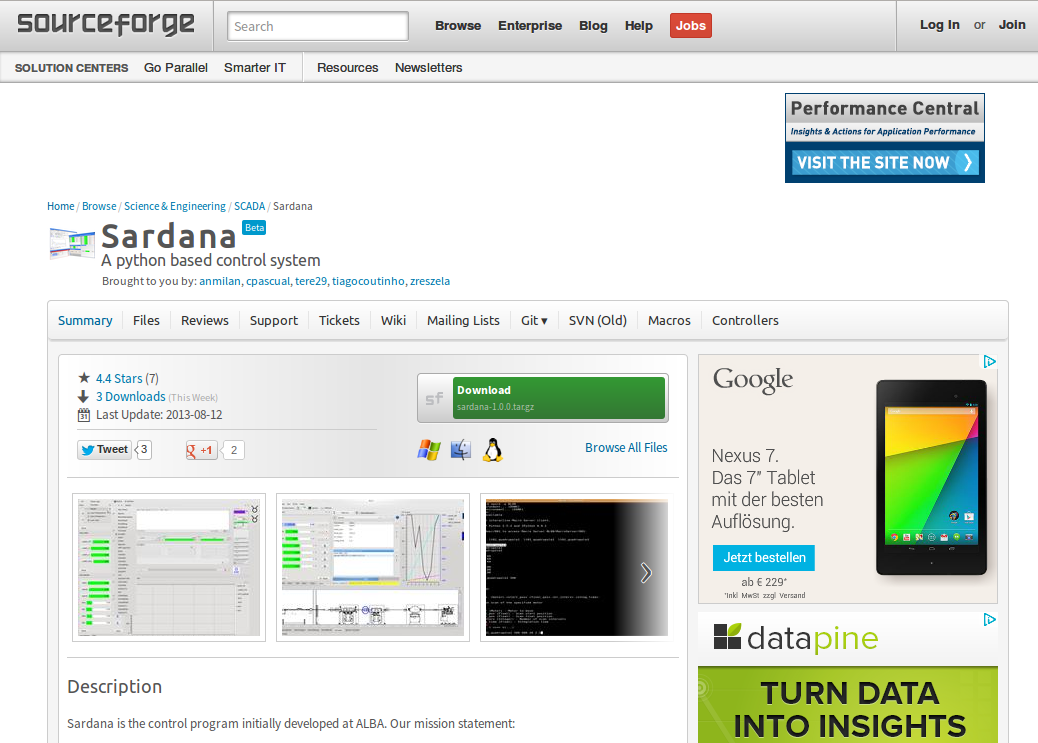
\includegraphics[width=4.0cm]{images/sf.png}
      \vspace{1em}
      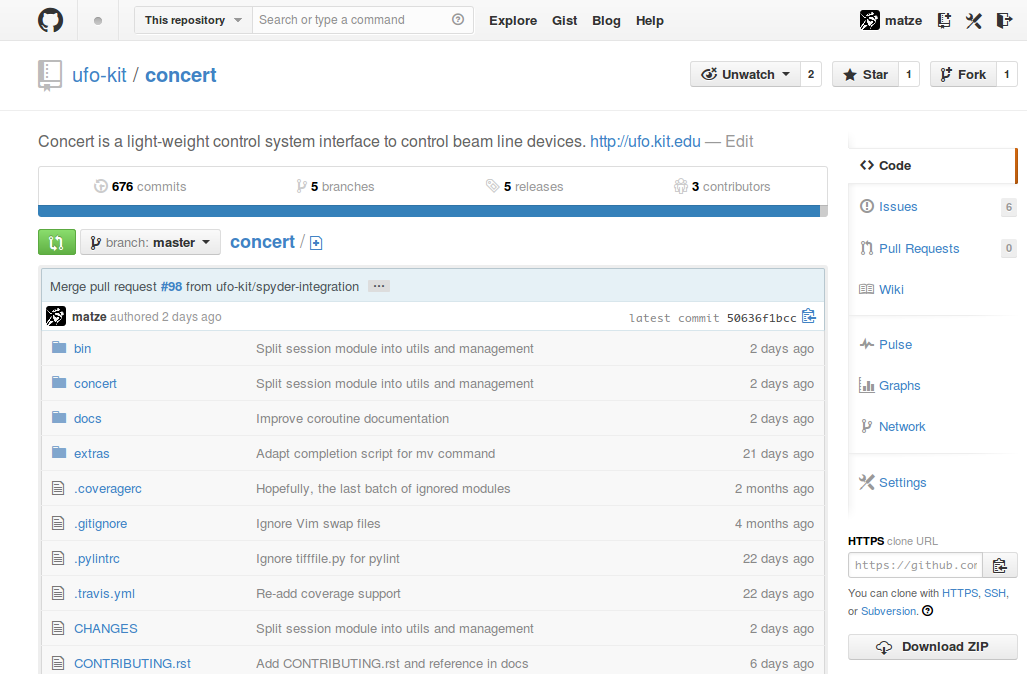
\includegraphics[width=4.0cm]{images/github.png}
  \end{columns}
\end{frame}

\section{Hands-on introduction}

\begin{frame}{}
  \begin{center}
    \huge\bfseries
    \textcolor{KITblack}{Git basics}
  \end{center}
\end{frame}
%\begin{frame}{Getting started}
  %\begin{block}{Installation}
    %\begin{itemize}
      %\item Debian/Ubuntu: \texttt{apt-get install git-core}
      %\item openSUSE/SLES: \texttt{zypper install git-core}
      %\item Fedora/RHEL/CentOS/SL: \texttt{yum install git}
      %\item Mac: \texttt{port install git-core} or install from
      %\url{http://git-scm.com/download/mac}
      %\item Windows: install from \url{http://git-scm.com/download/win}
    %\end{itemize}
  %\end{block}
%\end{frame}

\begin{frame}{Commits}
  Everytime you make a major change, you create a \alert{commit} containing:
  \begin{itemize}
    \item added/removed lines in files
    \item a comment summarizing what was changed
    \item an author
    \item a date
    \item a checksum (SHA-hash)
    \item a reference to the previous state of your files (parent(s))
  \end{itemize}
\end{frame}

\begin{frame}{Commit Graphs}
  Since most commits have a parent, they form a \alert{directed graph} without
  cycles (DAG).

  \begin{itemize}
    \item The first commit does not have a parent. It creates a \alert{repository}.
    \item Multiple commits can have the same parent (e.g. when coworkers work on the same code).
    \item Commits can have multiple parents if the two diverging changes are merged.
    \item Commits can have \alert{labels}. Labels can be e.g. branch names version tags.
  \end{itemize}
\end{frame}

\begin{frame}{Single User Workflow}
  \begin{enumerate}
    \item Create a repository
      \begin{shell}
        \$ git init
      \end{shell}
    \item Create a commit
      \begin{enumerate}
        \item Add something to the commit
          \begin{shell}
            \$ git add README.txt
          \end{shell}
        \item Perform the commit
          \begin{shell}
            \$ git commit -m "Added a README file"
          \end{shell}
      \end{enumerate}
  \end{enumerate}
\end{frame}

\begin{frame}{Single User Workflow}
  \begin{enumerate}
    \item Change something, and inspect the difference to the last commit
      \begin{shell}
        \$ vi README.txt\\
        \$ git diff\\
      \end{shell}
    \item Create a commit (as before)
      \begin{enumerate}
        \item Add some changes to the commit
          \begin{shell}
            \$ git add README.txt
          \end{shell}
        \item Perform the commit
          \begin{shell}
            \$ git commit -m "Added Copyright notice to README"
          \end{shell}
      \end{enumerate}
  \end{enumerate}
\end{frame}

\begin{frame}{When to commit}
  \begin{itemize}
    \item Small logical units
    \item About 3 times an hour
    \item Allows you to retrace your steps
  \end{itemize}
\end{frame}

\begin{frame}{Branching}
  \begin{itemize}
    \item Working on independent features at the same time
    \item Trying incompatible changes
    \item Quick and dirty work for a paper
  \end{itemize}
\end{frame}

\begin{frame}{Branching}
  \begin{itemize}
    \item Create two branches from master
      \begin{shell}
        \$ git checkout master\\
        \$ git checkout -b featureA\\
        \$ ...change \& commit something\\
        \$ git checkout -b featureB\\
        \$ ...change \& commit something
      \end{shell}
    \item Switch back to master branch
      \begin{shell}
        \$ git checkout master
      \end{shell}
    \item Merge your changes into master
      \begin{shell}
        \$ git merge featureA  \# fast forward\\
        \$ git merge featureB  \# merge
      \end{shell}
  \end{itemize}
\end{frame}

\begin{frame}{Retracing Your Steps}
  \begin{enumerate}
    \item Check the log
      \begin{shell}
        \$ git log  \# copy the SHA-key
      \end{shell}
    \item Show changes to current version
      \begin{shell}
        \$ git diff <paste SHA key>
      \end{shell}
    \item Check out old version
      \begin{shell}
        \$ git checkout <paste SHA key>
      \end{shell}
    \item Note that this does \emph{not change your branch}
  \end{enumerate}
\end{frame}


\begin{frame}{Creating a new repository}
  In the working directory of your project, type
  \begin{shell}
    \$ git init
  \end{shell}
\end{frame}
\begin{frame}{Tracking files}
  \begin{shell}
    \$ git add <path>
  \end{shell}
\end{frame}
\begin{frame}{Committing changes}
  \begin{shell}
    \$ git commit
  \end{shell}
\end{frame}
\begin{frame}{Excursion: File states}
  \begin{figure}
    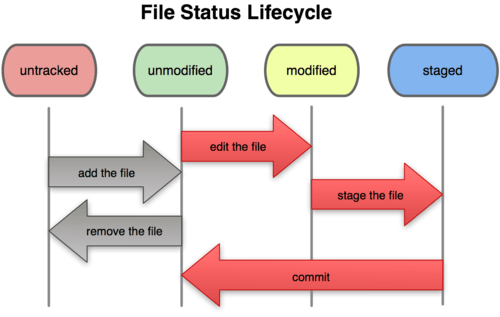
\includegraphics[width=9cm]{images/files}
    \caption{from Scott Schacon's \enquote{Pro Git} CC-BY-NC-SA 3.0}
  \end{figure}
\end{frame}
\begin{frame}{Checking the status}
  \begin{shell}
    \$ git status
  \end{shell}
\end{frame}
\begin{frame}{Staging changes}
So, before committing you have to stage a file
  \begin{shell}
\$ vi paper.tex\\
\$ git add paper.tex\\
\$ git commit
  \end{shell}
  or in one go
  \begin{shell}
    \$ git commit -a
  \end{shell}
\end{frame}
\begin{frame}{Visualizing the history}
  \begin{block}{For a quick look}
    \begin{shell}
      \$ git log
    \end{shell}
  \end{block}

  \begin{block}{GUIs}
    \begin{itemize}
      \item gitg
      \item gitk
      \item giggle
      \item tig
      \item \ldots
    \end{itemize}
  \end{block}
\end{frame}
\begin{frame}{Branches}
  \begin{columns}[onlytextwidth]
    \column{0.7\textwidth}
      To explore an idea without messing with the
      original work, you can create a branch off of it \ldots

      \begin{shell}
        \$ git branch fancy-idea\\
        \$ git checkout fancy-idea
      \end{shell}

      \visible<2->{
        and commit changes related to that idea
        \begin{shell}
          \$ git commit \ldots
        \end{shell}
      }

      \visible<3->{
        Branches are cheap, so don't bother creating as many as you like.
      }

    \column{0.3\textwidth}
      \centering
      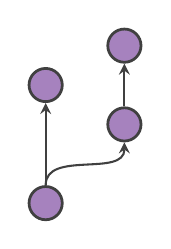
\begin{tikzpicture}
        \node[commit, circle, draw] (root) at (0,0) {};
        \visible<3->{
          \node[commit] (c1) at (0,1.5) {};
        }

        \visible<2->{
          \node[commit] (b1) at (1,1) {};
          \node[commit] (b2) at (1,2) {};
          \draw (root.north) edge[connection, out=90, in=270] (b1.south);
          \draw[connection] (b1) -- (b2);
        }

        \visible<3->{
          \draw[connection] (root) -- (c1);
        }
      \end{tikzpicture}
  \end{columns}
\end{frame}
\begin{frame}{Merging changes}
  \begin{columns}[onlytextwidth]
    \column{0.7\textwidth}
      If your changes are ready for prime time, merge them into your master
      branch:

      \visible<2->{
        \begin{shell}
          \$ git checkout master\\
          \$ git merge fancy-idea
        \end{shell}

        In this particular case, a \emph{merge commit} will be created.
      }

      \visible<3->{
        \vspace{1em}
        If merging was successful, the old branch can be removed

        \begin{shell}
          \$ git branch -D fancy-idea
        \end{shell}
      }

    \column{0.3\textwidth}
      \centering
      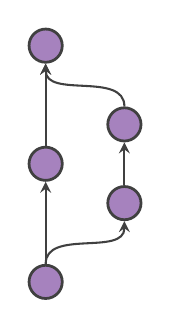
\begin{tikzpicture}
        \node[commit, circle, draw] (root) at (0,0) {};
        \node[commit] (c1) at (0,1.5) {};
        \node[commit] (b1) at (1,1) {};
        \node[commit] (b2) at (1,2) {};

        \draw (root.north) edge[connection, out=90, in=270] (b1.south);
        \draw[connection] (root) -- (c1);
        \draw[connection] (b1) -- (b2);

        \visible<2->{
          \node[commit] (c2) at (0,3) {};
          \draw (b2.north) edge[connection, out=90, in=270] (c2.south);
          \draw[connection] (c1) -- (c2);
        }
      \end{tikzpicture}
  \end{columns}
\end{frame}
\begin{frame}{Collaborating with others}
  \begin{itemize}
    \item Until now, everything happened on our local machine
    \item To share changes with others you can
      \begin{itemize}
        \item Send patches
        \item \emph{pull} from a remote repository
        \item \emph{push} from a remote repository
      \end{itemize}
    \item Remotes does not have to be a single server instance
    \item Different workflows can be easily modeled
  \end{itemize}
\end{frame}
\begin{frame}{Remote repositories}
  \begin{block}{Cloning repositories}
    \begin{shell}
      \$ git clone \{file,ssh,https\}://foo.server.com/foo.git
    \end{shell}
  \end{block}

  \begin{block}{Adding additional repositories}
    \begin{shell}
      \$ git remote add foo https://foo.server.com/foo.git
    \end{shell}
  \end{block}

  \begin{block}{Syncing changes}
    \begin{shell}
      \$ git pull [<remote> <branch>]\\
      \$ git push [<remote> <local-branch>:<remote-branch>]
    \end{shell}
  \end{block}
\end{frame}
%\begin{frame}{Hosting repositories}
  %\begin{itemize}
    %\item Some directory on a file share such as NFS
    %\item Simple SSH-based access or Gitolite
    %\item Third-party provider, e.g. GitHub, Bitbucket, Google Code,
      %SourceForge\ldots
  %\end{itemize}
%\end{frame}
%\begin{frame}{Best practices}
  %\begin{itemize}
    %\item Write descriptive commit messages and keep 50/70 limits
    %\item Check the status before committing
    %\item Think twice before running
      %\begin{shell}\$ git commit -a\end{shell}
  %\end{itemize}
%\end{frame}

\section{Advanced Git features}

\begin{frame}{}
  \begin{center}
    \huge\bfseries
    \textcolor{KITblack}{Advanced Git operations}
  \end{center}
\end{frame}
\begin{frame}{Manipulating the Git object database}
  If you collaborate heavily with your peers, you'll want to have a
  \enquote{clean} history of changes, e.g.

  \begin{itemize}
    \item Concise commit messages
    \item One commit per logical change
    \item A series of commits leading to a bigger change
  \end{itemize}
\end{frame}
\begin{frame}{Fixing the last commit}
  \begin{block}{Change author and message}
    \begin{shell}
      \$ git commit --amend
    \end{shell}
  \end{block}
\end{frame}
\begin{frame}{Picking cherries}
  \begin{block}{Pull individual commits into a branch}
    \begin{shell}
      \$ git cherry-pick f023bac
    \end{shell}
  \end{block}
\end{frame}
\begin{frame}{Partial staging}
  \begin{block}{Staging only relevant parts of a change}
    \begin{shell}
      git add -p/--patch
    \end{shell}
  \end{block}
\end{frame}
\begin{frame}{Stash intermediate changes away}
  \begin{block}{Cleaning the working directory temporarily}
    \begin{shell}
      \$ git stash "Descriptive message"\\
      \$ ... do something else\\
      \$ git stash pop
    \end{shell}
  \end{block}
\end{frame}
\begin{frame}{Merge bubbles}
  Merging branches that developed independently can end up nasty \ldots

  \begin{figure}
    \centering
    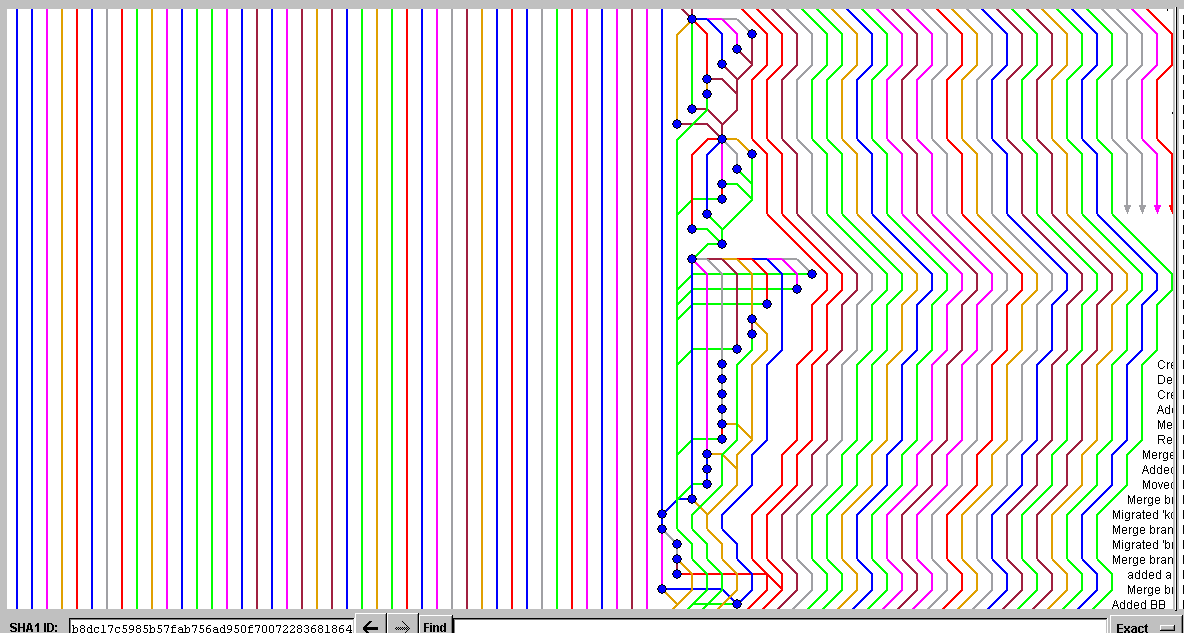
\includegraphics[width=8cm]{images/wide-gitk}
    \caption{\enquote{Successful} octopus merge.}
  \end{figure}
  \vfill
  {\footnotesize Image from: \url{http://blog.spearce.org/2007/07/difficult-gitk-graphs.html}}
\end{frame}
\begin{frame}{Rebasing branches}
  \begin{columns}[onlytextwidth]
    \column{0.7\textwidth}
    This can be reduced by rebasing one branch on top of the other
    \begin{shell}
      \$ git checkout some-feature\\
      \visible<2->{\$ git rebase master}
    \end{shell}
    \visible<3->{No merge commit, clean history.}

    \column{0.3\textwidth}
      \centering
      \begin{tikzpicture}

        \draw[connection] (root) -- (c1);
        \draw[connection] (b1) -- (b2);

        \visible<1>{
          \node[commit, circle, draw] (root) at (0,0) {};
          \node[commit] (c1) at (0,1.5) {};
          \node[commit] (c2) at (0,3) {};
          \node[commit, fill=syntax-number] (b1) at (1,1) {};
          \node[commit, fill=syntax-green!50] (b2) at (1,2) {};

          \draw[connection] (c1) -- (c2);
          \draw (root.north) edge[connection, out=90, in=270] (b1.south);
          \draw (b2.north) edge[connection, out=90, in=270] (c2.south);
        }

        \visible<2->{
          \node[commit, circle, draw] (root) at (0,0) {};
          \node[commit] (c1) at (0,1) {};
          \node[commit, fill=syntax-number] (b1) at (1,2) {};
          \node[commit, fill=syntax-green!50] (b2) at (1,3) {};
          \draw (c1.north) edge [connection, out=90, in=270] (b1.south);
        }

      \end{tikzpicture}
  \end{columns}
\end{frame}
\begin{frame}{Re-writing the history}
  \begin{columns}[onlytextwidth]
    \column{0.7\textwidth}
      Manipulate the change history by rebasing using the
      \texttt{-i/--interactive} switch

      \begin{itemize}
        \item \visible<2->{Drop commits}
        \item \visible<3->{Re-order commits}
        \item \visible<4->{Squash several commits into one}
        \item \visible<5->{Edit commits}
      \end{itemize}

      \visible<6->{
        \begin{shell}
        \$ git rebase -i HEAD\textasciitilde 4
        \end{shell}
      }

    \column{0.3\textwidth}
      \centering
      \begin{tikzpicture}
        % Drop commits
        \visible<1>{
          \node[commit] (c1) at (0,0) {};
          \draw[connection] (c1) -- (c2);
        }

        \visible<2->{
          \node[commit, opacity=0.5] (c1) at (0,0) {};
        }

        % Re-order commits
        \visible<1-2>{
          \node[commit, fill=syntax-number] (c2) at (0,1) {};
          \node[commit, fill=syntax-green!50] (c3) at (0,2) {};
        }

        \visible<3->{
          \node[commit, fill=syntax-green!50] (c2) at (0,1) {};
          \node[commit, fill=syntax-number] (c3) at (0,2) {};
        }

        % Squash commits
        \visible<1-3>{
          \node[commit, fill=KITgreen] (c5) at (0,4) {};
          \node[commit, fill=KITyellow] (c4) at (0,3) {};
          \draw[connection] (c4) -- (c5);
        }

        \visible<4->{
          \node[shape=circle split, commit,
                circle split part fill={KITgreen,KITyellow}] (c4) at (0,3)
              {\nodepart{lower}};
        }

        \draw[connection] (c2) -- (c3);
        \draw[connection] (c3) -- (c4);
      \end{tikzpicture}
  \end{columns}
\end{frame}
\begin{frame}{Best practices}
  \begin{itemize}
    \item Keep a clean history by re-writing the history of your local branch
    \item Never, ever re-write the history of a public branch (Once pushed,
      a change is sacred)
  \end{itemize}
\end{frame}


%\section{Beyond Source Control}

%\begin{frame}{}
  %\begin{center}
    %\huge\bfseries
    %\textcolor{KITblack}{Beyond version control}
  %\end{center}
%\end{frame}
%\begin{frame}{Deployment, Continous Integration}
  %\begin{block}{post-receive hooks}
    %\begin{description}
      %\item[what] Use post-receive hooks to trigger actions, e.g. running
        %builds and tests, deploy software, \ldots
      %\item[where] \texttt{\$REPO/.git/hooks}
      %\item[score]\score{1}{5}
    %\end{description}
  %\end{block}
%\end{frame}
%\begin{frame}{Blogging}
  %\begin{block}{GitHub pages + Jekyll}
    %\begin{description}
      %\item[what] Blog hosting on GitHub via Git and Jekyll
      %\item[where] \url{pages.github.com}
      %\item[score]\score{2}{5}
    %\end{description}
  %\end{block}
%\end{frame}
%\begin{frame}{Wiki}
  %\begin{block}{Gollum + Smeagol}
    %\begin{description}
      %\item[what] Git backend for a wiki with Markdown formatting
      %\item[where] \url{github.com/gollum/gollum} and
        %\url{github.com/rubyworks/smeagol}
      %\item[score]\score{2}{5}
    %\end{description}
  %\end{block}
%\end{frame}
%\begin{frame}{Backups}
  %\begin{block}{Bup}
    %\begin{description}
      %\item[what] Uses Git's packfile format to store backups
      %\item[where] \url{github.com/bup/bup}
      %\item[score]\score{2}{5}
    %\end{description}
  %\end{block}
%\end{frame}
%\begin{frame}{Managing large files}
  %\begin{block}{git-annex}
    %\begin{description}
      %\item[what] Manages large data sets across remotes
      %\item[where] \url{git-annex.branchable.com}
      %\item[score]\score{4}{5}
    %\end{description}
  %\end{block}
%\end{frame}
%\begin{frame}{Bug tracking}
  %\begin{block}{ticgit}
    %\begin{description}
      %\item[what] Keep tickets in a separate branch and sync across repos
      %\item[where] \url{github.com/jeffWelling/ticgit}
      %\item[score]\score{4}{5}
    %\end{description}
  %\end{block}
%\end{frame}
%\begin{frame}{Text-based slides}
  %\begin{block}{git-slides}
    %\begin{description}
      %\item[what] git-slides (together with Vim)
      %\item[where] \url{github.com/gelisam/git-slides}
      %\item[score]\score{5}{5}
    %\end{description}
  %\end{block}
%\end{frame}


\section{Appendix}

\begin{frame}{Further reads}
  \begin{columns}[T,onlytextwidth]
    \column{0.7\textwidth}
      \begin{itemize}
        \item \texttt{\$ man git} \ldots\  just kidding
        \item Free Pro Git book at \url{git-scm.com/book}
        \item Different aspects from beginners to pros: \url{gitready.com}
        \item Git cheat sheet: \url{ndpsoftware.com/git-cheatsheet.html}
        \item Interactive walkthrough: \url{gitimmersion.com}
      \end{itemize}

    \column{0.3\textwidth}
      \centering
      
\includegraphics[width=1.5cm]{images/pro-git}
      \vspace{2em}
      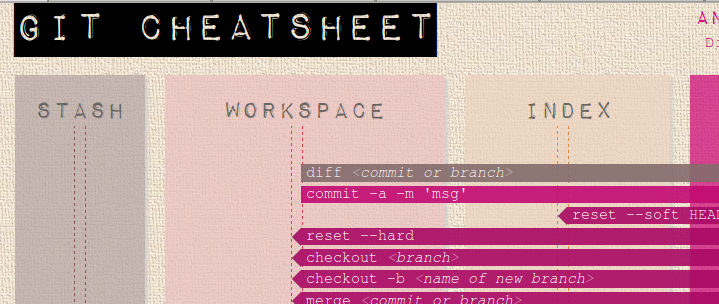
\includegraphics[width=3cm]{images/gcs}
  \end{columns}
\end{frame}
\begin{frame}{}
  \vfill
  \begin{center}
    \huge\bfseries
    \textcolor{KITblack}{Thanks for your attention!}
  \end{center}

  \vfill
  Get these slides from: \url{github.com/matze/kseta-dvsc-talk}\\
  Title logo by Jason Long licensed under CC-BY-3.0
\end{frame}

\end{document}

% vim:sw=2
